\documentclass[12pt]{article}
\usepackage[utf8]{inputenc}

\usepackage{amsmath,amssymb,amsthm}
\usepackage{graphicx}
\usepackage{float}
\usepackage[margin=1in]{geometry}
\usepackage{fancyhdr}
\usepackage{verbatim}
\usepackage{fancyvrb}
\usepackage{booktabs}
\usepackage{tabularx}
\usepackage{tikz}
\usetikzlibrary{automata, calc, positioning, shapes, shadows, arrows, fit, shapes.gates.logic.US, shapes.geometric}

%\title{Protues Malware Report}
%\author{Jason To-Tran}
%\date{23 April 2020}

\pagestyle{fancyplain}
\lhead{\textbf{To-Tran}}
\chead{\textbf{ECPE 293a} \\ Proteus Malware Report}
\rhead{\textbf{23 April 2020}}

\begin{document}\raggedright
\setlength{\parindent}{1em}
\setlength{\parskip}{1em}

\begin{titlepage}
	\begin{center}
		\vspace*{1cm}
		
		\textbf{Proteus Cryptocurrency Miner}
		
		\vspace{0.5cm}
		Malware Report
		
		\vspace{1.5cm}
		
		\textbf{Jason To-Tran}
		
		\vfill
		
		\vspace{0.8cm}
		
		% \includegraphics[width=0.4\textwidth]{university}
		
		ECPE 293a\\
		University of the Pacific\\

		23 April 2020
		
	\end{center}
\end{titlepage}

\subsection*{I. Executive Summary}

Proteus is a malware designed to exploit a system of its processing power and any sensitive information. This malware is capable of network communication to a webserver where it queries for specific files from said server. Since this is the case we can assume that following piece of malware was supposed to download a payload from the server to run. The piece of malware also performs changes to the registry so that it is able to auto-start when the infected computer reboots. I have also noticed that the malware runs programs that extracts system information from the computer. Possibly the worst part is how the malware is able to hide on the system and mask its true intentions.


In terms of detection, Proteus can be easily identified with the following signatures:

\begin{figure}[H]
	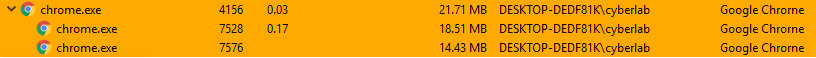
\includegraphics[width=\linewidth]{chrome_task.png}
	\caption{Google Chrome Processes}
	\label{fig:chrome_exe}
\end{figure}

\begin{figure}[H]\centering
	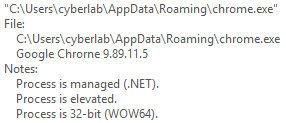
\includegraphics[width=3in]{chrome_details.png}
	\caption{Google Chrome Processes Details}
	\label{fig:chrome_details}
\end{figure}


In Figure \ref{fig:chrome_exe}, we can see several processes that appear to be Google Chrome. This is one sign that the following machine is infected with Proteus. Proteus disguises itself as a chrome.exe and runs in the background without the host noticing. The piece of malware even tries to appear that it is running from a "normal" location and this location is the user's \% APPDATA\% folder. Looking at the closer details in Figure \ref{fig:chrome_details}, we see the location in which the executable is being ran. Another interesting thing to note is the misspelling of "Google Chrorne 9.89.11.5". This is a dead give away that the following application is not legitimate. The notes portion of Figure \ref{fig:chrome_details}, continues to describe how the process is running. We can see that the process is managed by Microsoft NET Framework. This is very interesting since the legitimate version of Google Chrome does not require Microsoft NET Framework. In fact this was the one dependency that was needed to be installed on my virtual machine to get the malware running. To further drive home that the following is suspicious, the program is even running in elevated privileges which is very strange since Google Chrome is a browser and does not need those permissions. 

\begin{figure}[H]\centering
	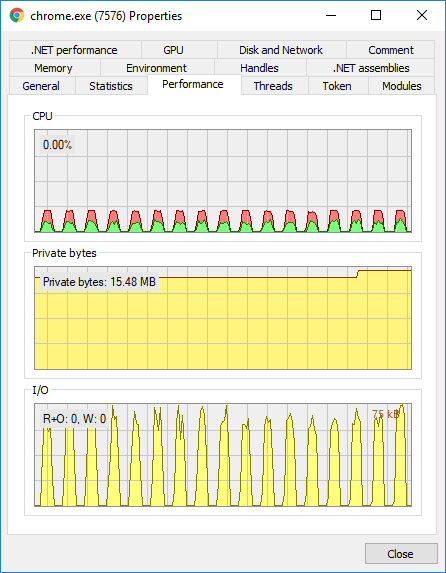
\includegraphics[width=3.25in]{chrome_pulse.png}
	\caption{Google Chrome Process Pulse for PID 7576}
	\label{fig:chrome_pulse}
\end{figure}


Looking at the process usage in Figure \ref{fig:chrome_pulse}, we can see a clock like pulse for both the CPU and the I/O. This behavior is only seen on one of the sub-processes for the malware. In my case we see this in the sub-process with PID: 7576. Another thing to note is that this is unlike any of the other processes running on my virtual machine and given that it is supposed to disguise itself as Google Chrome it should not be behaving like this. This could potentially means the program is communicating and sending computed messages to the command and control server.


In terms of data ex-filtration, the malware does an incredible job of hiding it from the user. This is shown in detail in the following figures:

\begin{figure}[H]\centering
	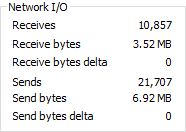
\includegraphics[width=2in]{chrome_net_proc.png}
	\caption{Google Chrome Network Process for PID 7576}
	\label{fig:chrome_net_proc}
\end{figure}

\newpage


\begin{figure}[H]\centering
	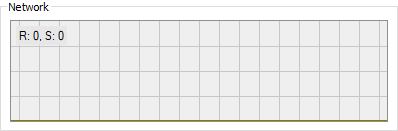
\includegraphics[width=5in]{chrome_network_graph.png}
	\caption{Google Chrome Network Graph for PID 7576}
	\label{fig:chrome_net_graph}
\end{figure}


As we can see in Figure \ref{fig:chrome_net_proc}, the malware is communicating over the network to the command and control server. Of course the command and control server is no longer running, so the received data is coming from Remnux. Apart from that, we can also see that the network graph for the process is not tracking any of the traffic coming from the malware. This is potentially due the malware interfacing with NET framework or using some obfuscated function to hide the traffic. Overall we cannot necessarily see what data is being taken since the command and control server is down, however we can further explore how this communication is done and what it is trying to send to the server. 


Overall, given this surface level knowledge of the malware, we know a general idea on how the attacker performs the attack. We know that the following malware is meant to infect a large amount of people so that they can be used for mining cryptocurrency. The malware has the potential to steal sensitive information from the user given that it downloads the correct payload from the command and control server. Since the malware is heavily reliant on the command and control server, it should not perform anything until making contact with the server. This makes it hard to reverse engineer the purpose of the malware since most of the operations given to the malware is from the server itself and if not given by the server the malware will not perform these tasks. It is also important to note that most of the functions are well obfuscated so this makes it extremely hard to determine what Windows API functions are being called and where. However, given the tell-tale signs of the malware we know that this is not aimed towards large corporate businesses. This malware is targeted more towards everyday individual users that are not too informed about security and networking.

\vspace*{\fill}
\noindent \textit{Note: The Executive Summary is a surface level analysis of the Proteus malware. It will describe general behavior that is understandable by most readers.}

\newpage

\subsection*{II. Identification}

% In this section, I will present the general identifiers for the malware in the following table:

\begin{figure}[H]
\begin{tabularx}{\linewidth}{|X|X|}
	\hline
	\textbf{Property} & \textbf{Value} \\
	\hline
	filenames & gchrome.exe
	\newline chrome.exe
	\newline Proteus.exe
	\newline pl.exe
	\newline 49FD4020BF4D7BD23956EA892E6860E9 
	\newline Proteus.....exe 
	\newline Proteus....exe  \\
	\hline
	file size & 2930176 bytes \\
	\hline
	md5 & 49FD4020BF4D7BD23956EA892E6860E9 \\
	\hline 
	sha1 & C5D8F155209BADD278437D0E534648F8- 
	\newline -D5C35AAE \\
	\hline
	sha256 & D23B4A30F6B1F083CE86EF9D8FF4340-
	\newline -56865F6973F12CB075647D013906F51A2 \\
	\hline 
\end{tabularx}
	\caption{Proteus Identification}
	\label{fig:proteus_indentification}
\end{figure}

\newpage

\subsection*{III. Capabilities}

\begin{figure}[H]\centering
	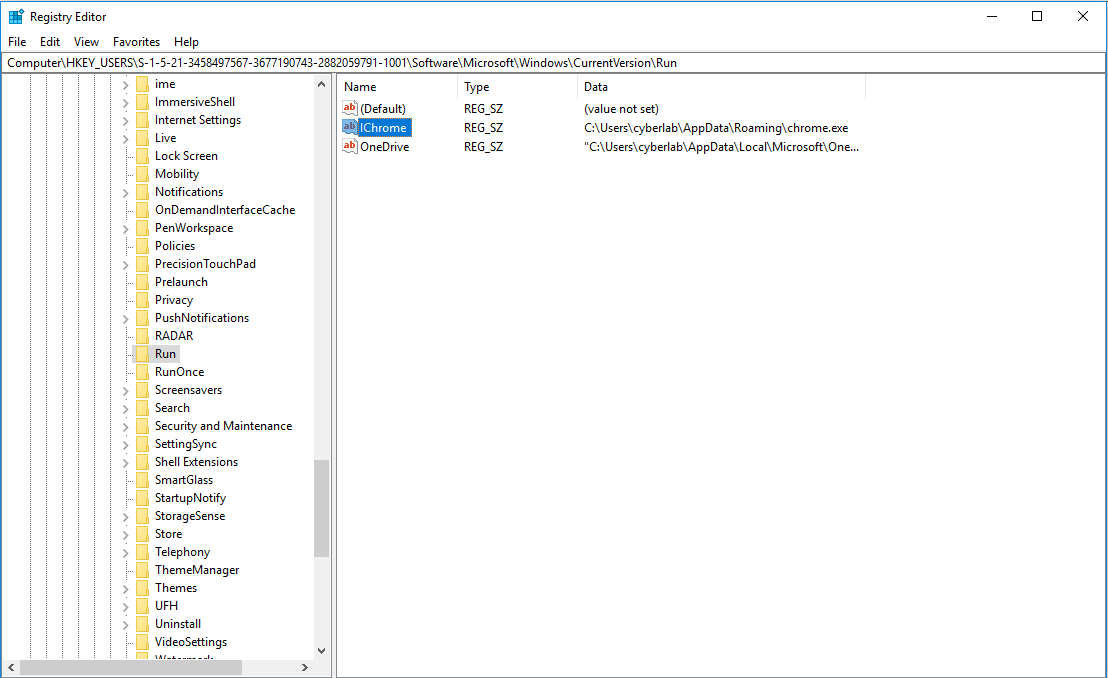
\includegraphics[width=6.5in]{registry_run.png}
	\caption{Regedit Run Key}
	\label{fig:reg_run}
\end{figure}

\begin{Verbatim}
HKU\S-1-5-21-3458497567-3677190743-2882059791-1001\Software\Microsoft\Windows\-
-CurrentVersion\Run\IChrome: "C:\Users\cyberlab\AppData\Roaming\chrome.exe"

HKU\S-1-5-21-3458497567-3677190743-2882059791-1001\Software\Microsoft\Windows\-
-CurrentVersion\Search\RecentApps\{34E52FA0-53F8-404C-9412-C3CCBFE31F24}\AppId-
-: "C:\Users\cyberlab\Desktop\proteus\PROTEUS\gchrome.exe"

HKU\S-1-5-21-3458497567-3677190743-2882059791-1001\Software\Microsoft\Windows -
-NT\CurrentVersion\AppCompatFlags\Compatibility Assistant\Store\C:\Users\cyber-
-lab\Desktop\proteus\PROTEUS\gchrome.exe:  53 41 43 50 01 00 00 00 00 00 00 00-
- 07 00 00 00 28 00 00 00 00 B6 2C 00 55 D6 2C 00 01 00 00 00 00 00 00 00 00 0-
-0 00 0A 71 22 00 00 DB 80 FD AC 28 39 D3 01 00 00 00 00 00 00 00 00

HKU\S-1-5-21-3458497567-3677190743-2882059791-1001\Software\Classes\Local Sett-
-ings\Software\Microsoft\Windows\Shell\MuiCache\C:\Users\cyberlab\Desktop\prot-
-eus\PROTEUS\gchrome.exe.FriendlyAppName: "Google Chrorne"
\end{Verbatim}

\newpage

\begin{figure}[H]
\begin{Verbatim}
HKU\S-1-5-21-3458497567-3677190743-2882059791-1001_Classes\Local Settings\Soft-
-ware\Microsoft\Windows\Shell\MuiCache\C:\Users\cyberlab\Desktop\proteus\PROTE-
-US\gchrome.exe.FriendlyAppName: "Google Chrorne"
\end{Verbatim}
	\caption{Proteus Registry Key Changes}
	\label{fig:proteus_registry_code}
\end{figure}


To begin, Proteus has the general malware ability to persist even when the computer is rebooted. The tool used to obtain this information was regshot, which helped identify registry values changed/added and files that were created. The autostart was done through a registry key edit made in the following location:

\begin{Verbatim}
HKU\S-1-5-21-3458497567-3677190743-2882059791-1001\Software\Microsoft\Windows\-
-CurrentVersion\Run\IChrome: "C:\Users\cyberlab\AppData\Roaming\chrome.exe"
\end{Verbatim}

\noindent Essentially this location in the registry is where you can add programs that will autostart when the computer starts up. By adding an entry to this location in registry, Proteus will be able to run right when the user logs in. The malware also seems to add itself to recently used programs. This is likely to trick the user into assuming that they have installed Google Chrome or somesort of Google Chrome plugin. The third registry entry is made in the Compatibility Assistant section of the registry. This is most likely to include compatibility flags to run the program properly. Finally the malware adds the friendly application name: "Google Chrorne" which is a dead give away that the host has been infected with some sort of malware. 


In terms of the potential to infect other files, Proteus has not been seen to show this functionality. And even when running the malware, ProcDot was not able to capture such behavior at runtime. Since this is the case, it has also not been seen to infect other devices on the network. What has been seen from the malware is its network communication and potential for stealing data and other sensitive information. With the help of Wireshark and ProcDot I was able to capture all of the behavior that the malware does when trying to communicate with the command and control server. In order to obtain a ProcDot analysis, I first obtained a Process Monitor .CSV by running the malware and capturing the behavior with Process Monitor. This was also done in parallel with Wireshark so that Procdot can sync the network communication with the all of the behavior captured on Process Monitor.


In the following figure, the files used to generate the procdot render are displayed:

\begin{figure}[H]\centering
	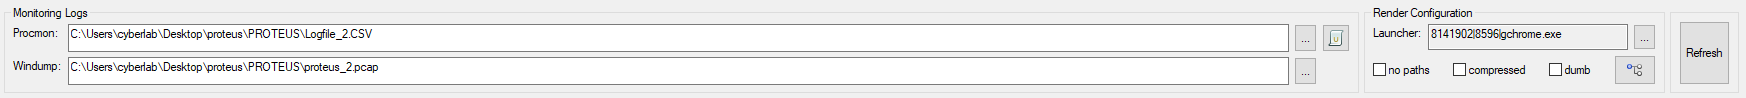
\includegraphics[width=\linewidth]{procdot_files.png}
	\caption{ProcDot Files}
	\label{fig:procdot_files}
\end{figure}

\begin{figure}[H]\centering
	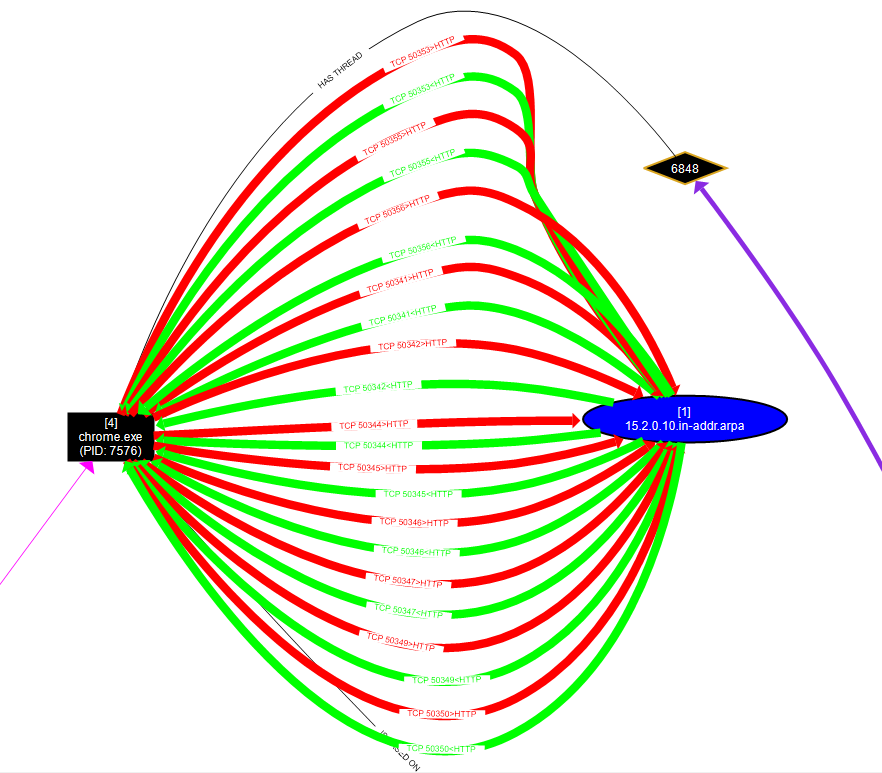
\includegraphics[width=6in]{proteus_procdot_net.png}
	\caption{Proteus ProcDot Network Communication}
	\label{fig:proteus_proc_net}
\end{figure}

For Figure \ref{fig:proteus_proc_net}, we can see Proteus send a lot of HTTP messages to the command and control server. In this case the command and control server is Remnux. The specific domain it is trying to communicate with is 15.2.0.10.in-addr.arpa. Another thing to notice about the malware is that it sending the packets from TCP port 50356 to 80. Researching the what services generally use port 50356 I found that it is used for the following services:

\begin{enumerate}
	\item Dynamic and/or Private Ports
	\item Xsan Filesystem
\end{enumerate}

\noindent Based on the following, I can make several assumptions about the malware. It appears that it is using this Apple specific port since the malware was created to run on Windows. Apart from that, this can be considered a signature that could potentially mean that a client is infected with Proteus since not a lot of applications would use this port for communication.

\begin{figure}[H]\centering
	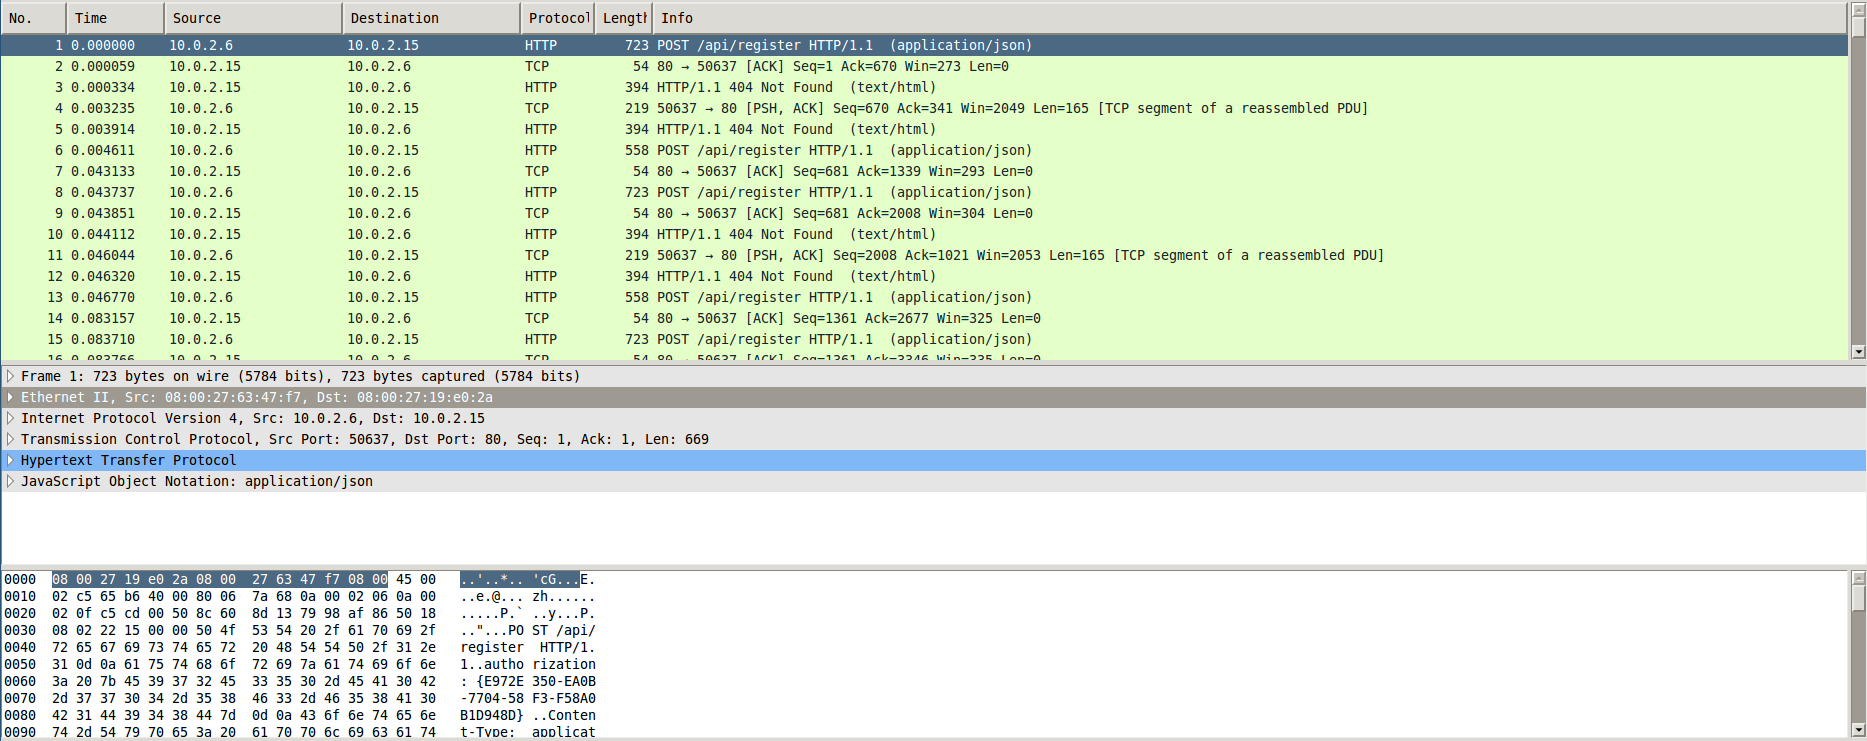
\includegraphics[width=6.5in]{wireshark_post_messages.png}
	\caption{Wireshark HTTP Messages from Proteus}
	\label{fig:wireshark_post_messages}
\end{figure}


From the following Wireshark Capture (from Remnux), we can see that the Proteus malware continually sends an HTTP Post message to the webserver. It appears to referrencing /api/register. I am assuming that the Proteus command and control server has some sort of API built to manage the infected hosts. It is also very important to look at the word register. When Proteus sends the command to the command and control server it is possibly asking the server to register the following device. Since the server does not respond, Proteus continues to send the message since it is unable to carry out other tasks without the server. This makes me wonder what is inside the HTTP Post messages. There could potentially be information on the commands or on what kind of application is being run on the server-side. Perhaps there are fields or other information that are embedded in the messages.

\begin{figure}[H]\centering
	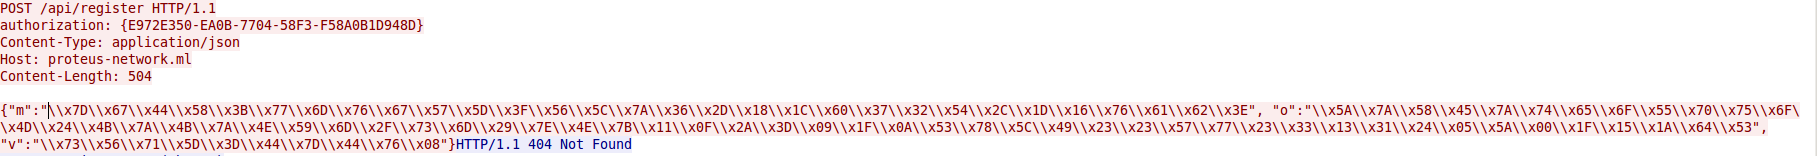
\includegraphics[width=\linewidth]{wireshark_tcp_follow.png}
	\caption{Proteus Message Fields}
	\label{fig:tcp_follow}
\end{figure}


In Figure \ref{fig:tcp_follow}, I used the follow TCP stream so that I was able to see the back and forth communication between Proteus and Remnux. What is worthy to note is that the message sent to the server has three distinct field: 'm', 'o' and 'v'. With in the field appears to be hex-values that could potentially provide clues on waht the following message is asking the command and control server to do. I then obtained the hex-values from each field and converted them to ascii to see whether it had any meaning. Upon doing so, I obtained values that looked like gibberish (this conversion of hex to ascii was done a website). This could potentially mean that the malware is encrypting the messages.


\noindent Converted message fields:

\begin{figure}[H]\centering
	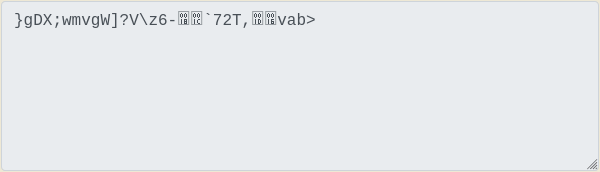
\includegraphics[width=6in]{m_message.png}
	\caption{'m' Field}
	\label{fig:m_message}
\end{figure}

\begin{figure}[H]\centering
	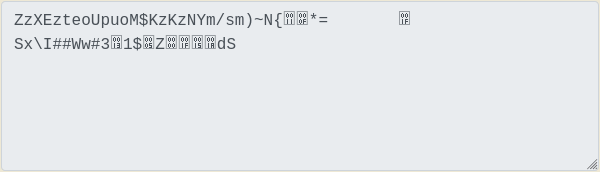
\includegraphics[width=6in]{o_message.png}
	\caption{'o' Field}
	\label{fig:o_message}
\end{figure}

\begin{figure}[H]\centering
	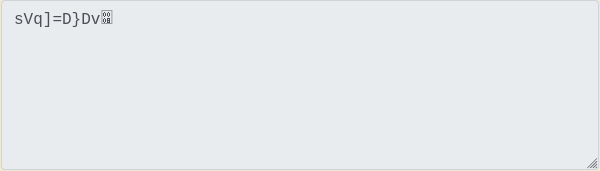
\includegraphics[width=6in]{v_message.png}
	\caption{'v' Field}
	\label{fig:v_message}
\end{figure}

\newpage

\begin{figure}[H]\centering
	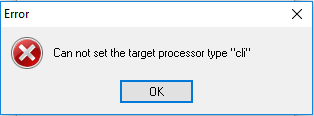
\includegraphics[width=4in]{cli_error.png}
	\caption{IDA Pro 'cli' Issue}
	\label{fig:cli_error}
\end{figure}

Proteus does something very interesting when hiding its functionality. In fact, I was very thrown off when I was examining it within the disassembler. Initially, I tried examining the executable in IDA however I ran into a very interesting issue. I believe that the free version of IDA Pro does not have compatibility towards Microsoft.Net assembly. Since this was the case IDA played no help in determining what the malware was doing under the hood. Upon realizing this, I was forced to use x32dbg (since Proteus is a 32-bit malware) for all of the underlying assembly analysis. I did this initially to ensure that I was even able to use disassembler or debugger on the executable.


I then wanted to ensure that the malware was not packed, since this would make analyzing the executable more complicated. To do this I began using bytehist to look at a histogram of the bit frequency. If the histogram has a uniform bit frequency then that must mean that there is some form of packing that is used on the malware to hide its true functionality. The following is images of the bytehist histogram:

\begin{figure}[H]\centering
	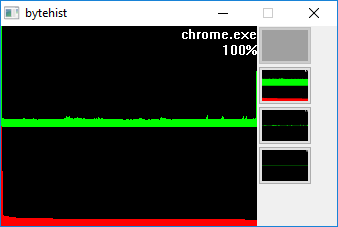
\includegraphics[width=5in]{chrome_bytehist.png}
	\caption{chrome.exe Byte Histogram}
	\label{fig:chrome_bytehist}
\end{figure}

\newpage

\begin{figure}[H]\centering
	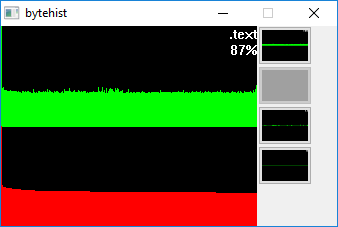
\includegraphics[width=5in]{text_bytehist.png}
	\caption{.text Byte Histogram}
	\label{fig:text_bytehist}
\end{figure}

\noindent As we can see from the byte histogram of both chrome.exe and .text, the bit frequency is strangely uniform. The malware could potentially be packed by Microsoft NET since it is in Microsoft.Net assembly. To further verify this, I turned towards Detect It Easy, EXEInfo PE. When running these on Proteus, I was given split results. Detect It Easy thought the program was not packed, however EXEInfo PE saw that the program was packed/obfuscated using Microsoft Visual Basic. The following figure is the output from EXEInfo PE:

\begin{figure}[H]\centering
	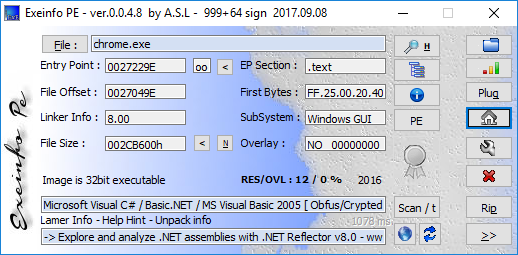
\includegraphics[width=6in]{exeinfo.png}
	\caption{EXEInfo PE Output}
	\label{fig:exeinfo}
\end{figure}

\noindent I wanted to verify further that the malware was truly packed, so I ran the Linux tools on it. Most of the tools found that the malware was not packed except for PEScan which returned the message that the malware was probably packed due to the entropy value. This was the command line message when running the tool:
 
\begin{figure}[H]
\begin{Verbatim}
remnux@remnux:~/dev/project_proposal$ pescan gchrome.exe 
file entropy:                    7.821597 (probably packed)
fpu anti-disassembly:            no
imagebase:                       normal
entrypoint:                      normal
DOS stub:                        normal
TLS directory:                   not found
section count:                   3
.text:                           normal
.rsrc:                           normal
.reloc:                          small length
timestamp:                       normal
\end{Verbatim}
\caption{PEScan Output}
\label{fig:pescan}
\end{figure}

\begin{figure}[H]\centering
	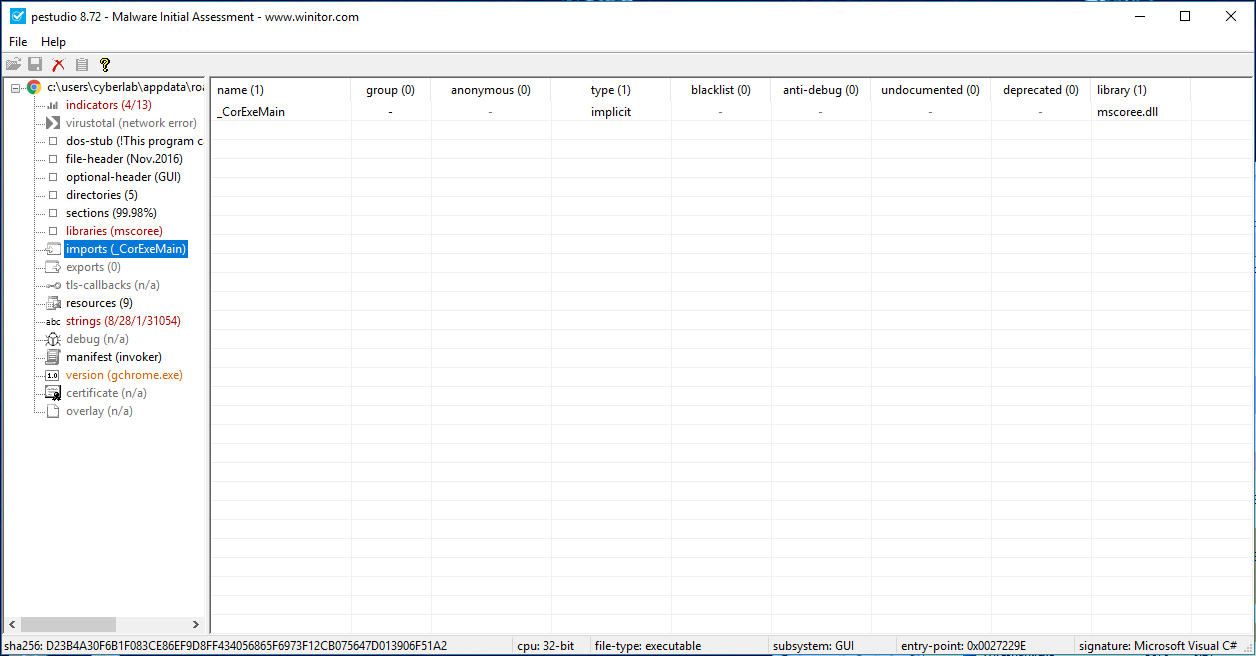
\includegraphics[width=5in]{pe_imports.png}
	\caption{PE Import Output}
	\label{fig:pe_imports}
\end{figure}


Overall, I can assume that the malware is not packed since most of the tools reported negative. From there I wanted to know whether the malware programmer made an effort into obfuscating the code and implementing any resistance to debuggers. Looking at the import scans using the PE tool, we can see that Proteus makes an effort to hide the Libraries and Windows API functions it is using to modify the system. When running the tool on a debugger we were ultimately not met with any anti-debugging measures.

\newpage

\begin{figure}[H]\centering
	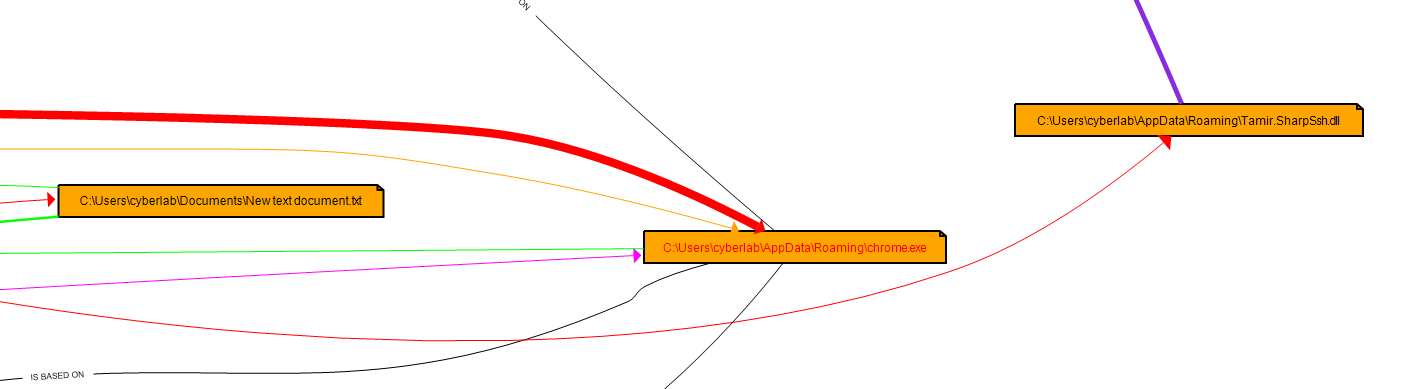
\includegraphics[width=6.5in]{file_dropping.png}
	\caption{File Dropping}
	\label{fig:file_dropping}
\end{figure}


As for miscellaneous capabilities, the Proteus malware is able to drop files onto the system and run/create processes. In Figure \ref{fig:file_dropping}, we can see on runtime that the malware is dropping three different files. The first file that was created is "New text document.txt" which is strangely used by SearchProtocolHost.exe. The next file created was chrome.exe in the following directory:

\begin{figure}[H]
\begin{Verbatim}
C:\Users\cyberlab\AppData\Roaming\chrome.exe
\end{Verbatim}
\caption{chrome.exe Directory}
\label{fig:chrome_directory}
\end{figure}

\noindent Upon creating the following file, the malware terminates itself and runs the executable in that location. The final file that is created is Tamir.SharpSsh.dll. Although this file is created, it is not seen within the import list provided by PE. Looking at the debugger, this is probably imported using the LoadLibrary function.

\newpage

\subsection*{IV. Dependencies}


As for dependencies, Proteus is a 32-bit windows based malware so it can run on either 32-bit or 64-bit versions of Windows. From what I can tell, the malware does not seem to be targetting a specific version of Windows. From the observed behavior, inorder for the malware to operate it requires an internet connection. It also requires a connection to the command and control server. The domain it contacts is proteus-network.ml, which seems to be down at the moment. A major dependency that the malware has is NET framework. In order to even run the malware, NET Framework 3.5 must be installed on this system. 


\subsection*{V. Indicators of Compromise}


\noindent \textbf{Indicators:}


\begin{enumerate}
\item Indicator: gchrome.exe 
	\begin{enumerate}
	\item Type: File 
	\item MD5: 49FD4020BF4D7BD23956EA892E6860E9
	\end{enumerate}
\item Indicator: C:\textbackslash Users\textbackslash cyberlab\textbackslash AppData\textbackslash Roaming\textbackslash chrome.exe
	\begin{enumerate}
	\item Type: File 
	\item MD5: 49FD4020BF4D7BD23956EA892E6860E9
	\end{enumerate}
\item Indicator: C:\textbackslash Users\textbackslash cyberlab\textbackslash AppData\textbackslash Roaming\textbackslash Tamir.SharpSsh.dll
	\begin{enumerate}
	\item Type: File 
	\item MD5: 2859F8073BC71C8A0331E46ECE0E6213
	\end{enumerate}
\item Indicator: C:\textbackslash Users\textbackslash cyberlab\textbackslash Documents\textbackslash New text document.txt
	\begin{enumerate}
	\item Type: File
	\item MD5: E4654597B12592C4A148957486CB2D55
	\end{enumerate}
\item Indicator: 15.2.0.10.in-addr.arpa
	\begin{enumerate}
		\item Type: Address
	\end{enumerate}
\item Indicator: proteus-network.ml
	\begin{enumerate}
		\item Type: Address
	\end{enumerate}
\item Indicator: HKU\textbackslash S-1-5-21-3458497567-3677190743-2882059791-1001\_Classes\textbackslash Local Settings\textbackslash Software\textbackslash Microsoft\textbackslash Windows\textbackslash Shell\textbackslash MuiCache\textbackslash C:\textbackslash Users\textbackslash cyberlab\textbackslash Desktop\textbackslash \newline proteus\textbackslash PROTEUS\textbackslash gchrome.exe.FriendlyAppName: "Google Chrorne"
	\begin{enumerate}
		\item Type: Registry
	\end{enumerate}
\item Indicator: HKU\textbackslash S-1-5-21-3458497567-3677190743-2882059791-1001\textbackslash Software\textbackslash Classes\textbackslash Local Settings\textbackslash Software\textbackslash Microsoft\textbackslash Windows\textbackslash Shell\textbackslash MuiCache\textbackslash C:\textbackslash Users\textbackslash cyberlab\textbackslash Desktop\textbackslash \newline proteus\textbackslash PROTEUS\textbackslash gchrome.exe.FriendlyAppName: "Google Chrorne"
	\begin{enumerate}
		\item Type: Registry 
	\end{enumerate}
\item Indicator: HKU\textbackslash S-1-5-21-3458497567-3677190743-2882059791-1001\textbackslash Software\textbackslash Microsoft\textbackslash Windows NT\textbackslash CurrentVersion\textbackslash AppCompatFlags\textbackslash Compatibility Assistant\textbackslash Store\textbackslash C:\textbackslash Users\textbackslash cyberlab\textbackslash Desktop\textbackslash proteus\textbackslash PROTEUS\textbackslash gchrome.exe:  53 41 43 50 01 00 00 00 00 00 00 00 07 00 00 00 28 00 00 00 00 B6 2C 00 55 D6 2C 00 01 00 00 00 00 00 00 00 00 00 00 0A 71 22 00 00 DB 80 FD AC 28 39 D3 01 00 00 00 00 00 00 00 00
	\begin{enumerate}
		\item Type: Registry
	\end{enumerate}
\item 
HKU\textbackslash S-1-5-21-3458497567-3677190743-2882059791-1001\textbackslash Software\textbackslash Microsoft\textbackslash Windows\textbackslash CurrentVersion\textbackslash Search\textbackslash RecentApps\textbackslash\{ 34E52FA0-53F8-404C-9412-C3CCBFE31F24\}\textbackslash AppId: "C:\textbackslash Users\textbackslash cyberlab\textbackslash Desktop\textbackslash proteus\textbackslash PROTEUS\textbackslash gchrome.exe"
	\begin{enumerate}
		\item Type: Registry
	\end{enumerate}
\item HKU\textbackslash S-1-5-21-3458497567-3677190743-2882059791-1001\textbackslash Software\textbackslash Microsoft\textbackslash Windows\textbackslash CurrentVersion\textbackslash Run\textbackslash IChrome: "C:\textbackslash Users\textbackslash cyberlab\textbackslash AppData\textbackslash Roaming\textbackslash chrome.exe"
	\begin{enumerate}
		\item Type: Registry
	\end{enumerate}
\end{enumerate}


\noindent \textbf{Importance:}


In the first entry in the list of indicators, the following file is the initial executable that runs the malware. This is important since it is the initial sign of compromise so it would be very important to take note of the MD5 hash. The second entry is the file dropped by the malware. Upon creating this file, the initial process is terminated and it will run the following executable. Once the process is started, the malware will create subprocesses from that executable. The Tamir.SharpSsh.dll contains functions that are used by the executable. Based on online resources, Tamir.SharpSsh.dll contains Windows API functions pertaining to secure shell. Finally, the last file is used for the application: SearchProtocolHost.exe.  


Moving onto the addresses listed in the indicators, the malware performs a DNS query for 15.2.0.10.in-addr.arpa. After completing the DNS query, Proteus tries to communicate with the command and control server. The command and control server has the domain: proteus-network.ml. The malware then communicates with the server with a HTTP post requeset for /api/register. This register file was probably used to register the following computer so that it can be used as a miner or as an ID so that the attacker can steal information from the user.


The last of the indicators are the registry keys that were added/editted by Proteus. In the 7th and 8th indicators, the malware is applying a name onto the process. I believe it is trying to mask itself as Google Chrome, however, it is mispelled. The 9th indicator is compatibility flags written for gchrome.exe. The 10th indicator is the registry referring to recently used apps. This simply adds gchrome.exe to that list. Finally the run key will automatically start the malware when the user logs in.


\noindent \textbf{Tools used to Obtain Indicators:}


\begin{enumerate}
	\item RegShot
	\item Process Monitor 
	\item Wireshark 
	\item TcpLogView
	\item ProcDOT
	\item x32dbg (Refer to Behavioral and Code Analysis Documentation)
\end{enumerate}
\newpage 


\subsection*{VI. Behavioral and Code Analysis Documentation}


Since I have discussed the tools I have used to investigate the behavior of the malware, I will focus more on the code analysis. I believe the most interesting aspect of Proteus is the way in which it obfuscates both its function calls and strings. Analyzing the behavior of the malware alongside the assembly was incredibly difficult since all of the function calls were hidden. Proteus actually manages to bypass the general LoadLibrary and GetProcAddress functions (these are still present in the code although the programmer is using a different method to hide them). Once I ran the debugger I noticed I was not within the chrome.exe .text portion of the assembly. The code began in the ntdll.dll which was very interesting. Since this was the case I wanted to do some investigation on the functions within ntdll.dll.


Doing some research online, I found out that ntdll.dll contain functions that interface with the Windows kernel. These function calls are lower-level compared to the average Windows API calls that are used. Due to this, it hard to distinguish what functions are being called since most of the function called were done through ordinal numbers. I believe if I can figure out the ordinal numbers from the code it will really help in the reverse engineering process. In order to figure out the functions within ntdll.dll I needed to run it within a dissassembler. So my first task was to find the location of ntdll.dll. I made a general guess that the file was located in the system32 directory. This turned out to be true; the following is the directory to ntdll.dll: 

\begin{figure}[H]
\begin{Verbatim}
C:\Windows\System32\ntdll.dll
\end{Verbatim}
\caption{ntdll.dll Directory}
\label{fig:ntdll_dir}
\end{figure}

\noindent From there I ran IDA and examined the functions that were included in ntdll.dll. In the following figure IDA displays the function names and ordinal numbers for each function within the dll:

\begin{figure}[H]\centering
	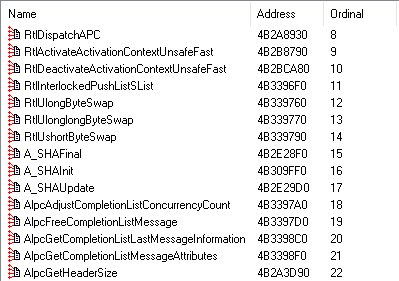
\includegraphics[width=3.5in]{ida_ntdll.png}
	\caption{IDA ntdll.dll}
	\label{fig:ida_ntdll}
\end{figure}


\newpage 

\begin{figure}[H]\centering
	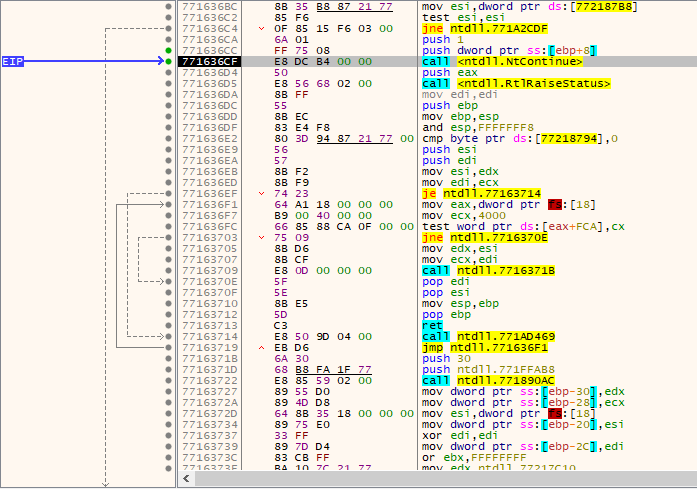
\includegraphics[width=3.25in]{ntcontinue.png}
	\caption{x32dbg NTContinue}
	\label{fig:ntcontinue}
\end{figure}

Moving onto analyzing the code for chrome.exe, the only debugger I was able to run on it was x32dbg. Once I ran the debugger, I was located in the ntdll.dll portion of the assembly. This was very strange and it was hard to distinguish what functions were being called since the function calls were all addresses with no real distinguishable identifiers. At this point, I wanted to figure out how the malware was creating new sub-processes. Since I was not too sure about how the ntdll.dll function calls were occuring I decided to step through the code to grab some bearings. Running through the assembly, I noticed a portion where the program seemed to "freeze". In Figure \ref{fig:ntcontinue}, we can see the function call that occurs when the program appears to freeze. After "freezing" (performing some sort of operation to launch the sub-process), the program counter jumps to the following location in the code: 

\begin{figure}[H]\centering
	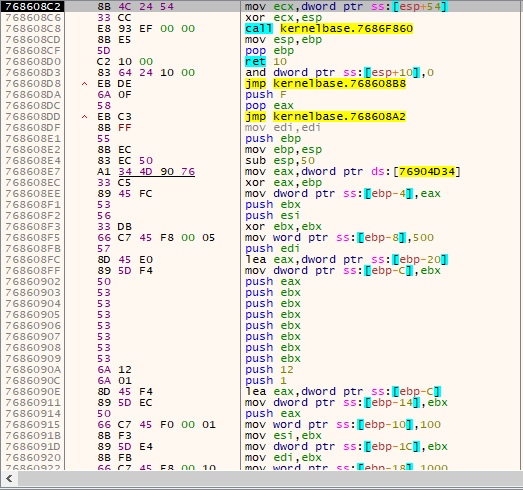
\includegraphics[width=3.25in]{ntcontinue_aftermath.png}
	\caption{x32dbg NTContinue Jump}
	\label{fig:ntcontinue_return}
\end{figure}

\newpage

\begin{figure}[H]\centering
	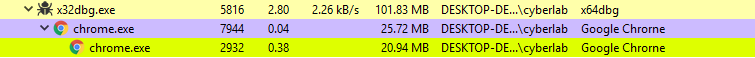
\includegraphics[width=\linewidth]{new_subprocess.png}
	\caption{Task Manager chrome.exe}
	\label{fig:new_subprocess}
\end{figure}

Take note that the address it jumps to is the kernelbase.dll section. This is probably due to ntdll.dll interfacing with the Windows kernel. However after completing the instruction and jump a new process appeared in the taskmanager, which means that something was occuring in the ntdll.dll where it is able to create a new sub-processes. Figure \ref{fig:new_subprocess}, displays the new chrome.exe subprocess after executing the NTContinue function. This is repeated for the second sub-process, where the executable sends HTTP messages to the server. Since there are multiple sessions of chrome.exe performing different portions of the assembly, it would be very nice to examine the other processes. It turns out that x32dbg has the ability to attach to the other subprocesses which allows me to examine what they are doing. In the image below x32dbg shows the option to attach to the other chrome.exe sub-processes:

\begin{figure}[H]\centering
	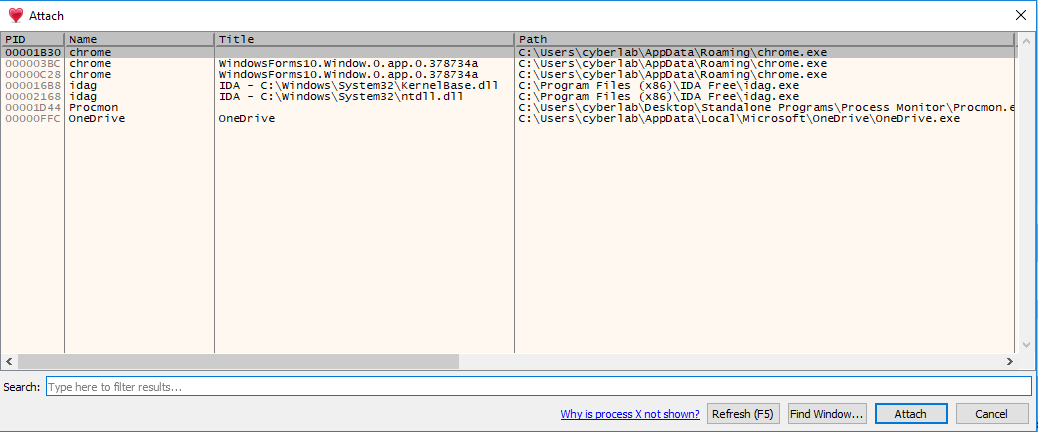
\includegraphics[width=\linewidth]{x32dbg_other_proc.png}
	\caption{x32dbg Other Processes}
	\label{fig:x32dbg_other_proc}
\end{figure}

To ensure that the sub-process is not replaced, I opened three sessions of x32dbg and attached it to each chrome.exe process. After attaching x32dbg to the last chrome.exe process (the last subprocess), the network communication from the malware seemed to stop. That means the last sub-process created is managing the network communcation and potentially creating/encyrpting the messages. The figure below displays wireshark only receiving Windows service related messages (all communication from the malware has ceased):

\newpage

\begin{figure}[H]\centering
	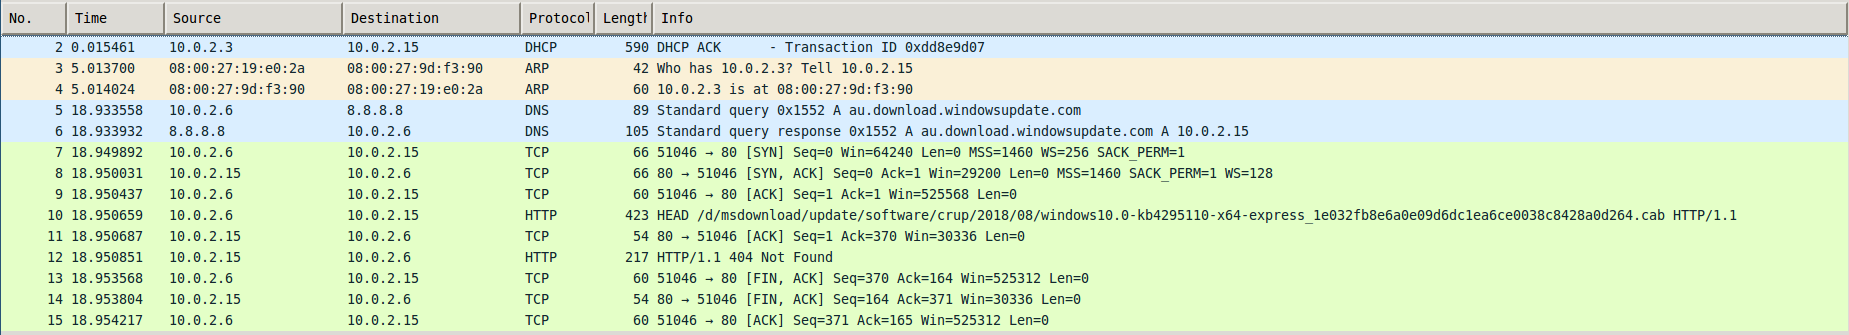
\includegraphics[width=\linewidth]{wireshark_x32dbg_test.png}
	\caption{Wireshark only Receiving Windows Related Network Communication}
	\label{fig:wireshark_x32dbg}
\end{figure}


At this point, I wanted to know the general location where the network communication was occuring. To do this I had Remnux and the infected Windows machine running side-by-side. The Remnux machine was monitoring the network traffic and the Windows machine was running the debugger. To force the network communication I stepped through the code until I reached a block of code that was sending out the HTTP messages. I knew that this shouldn't be a very long process since the main purpose of this process was to communicate to the command and control server. The following image is my setup to perform this test:

\begin{figure}[H]\centering
	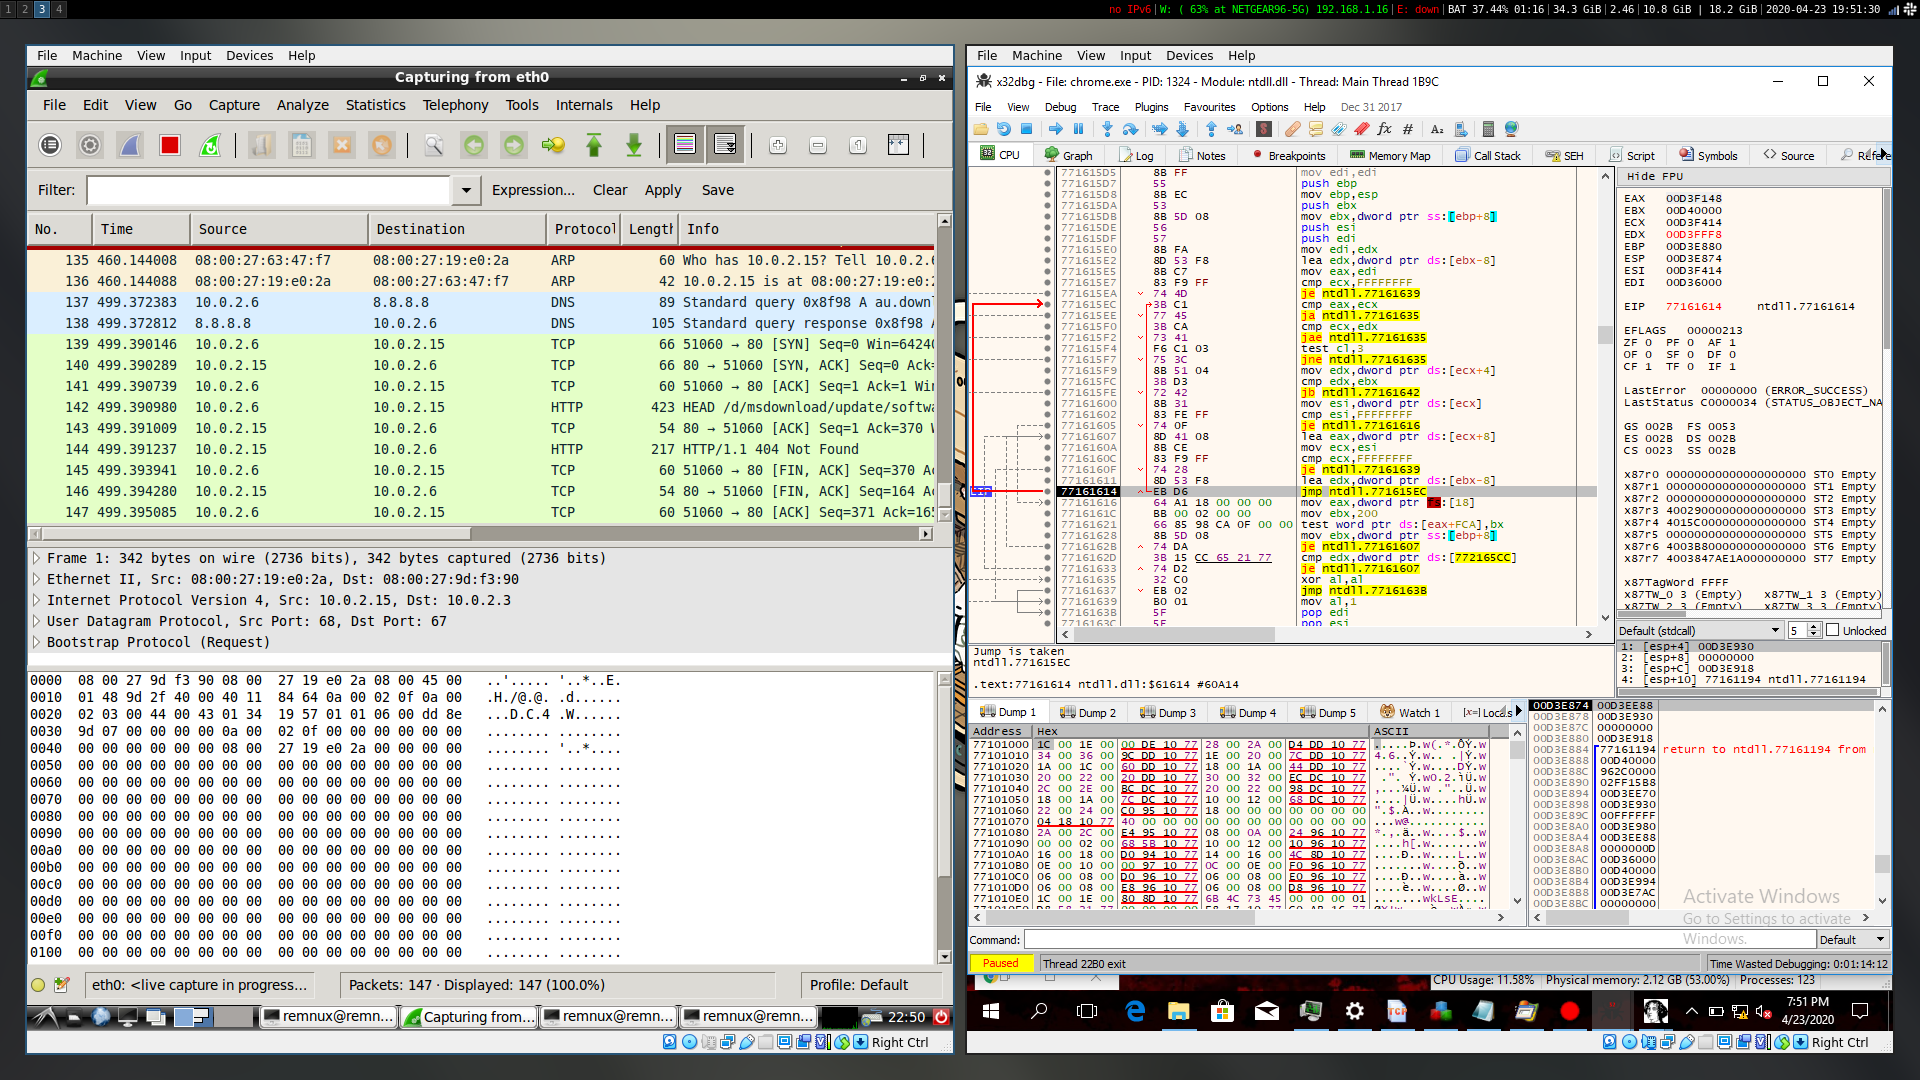
\includegraphics[width=\linewidth]{workflow_for_debugging_net.png}
	\caption{Workflow for Understanding Malware Network Communication}
	\label{fig:net_comm_workflow}
\end{figure}

\noindent Although this is a very hacking way of understand what the code does, it helped me work around the ntdll.dll obfuscation. By doing this I learned that the malware runs through the code three times to prepare the message. After preparing the message it will send the message on the fourth loop. After realizing this, I was able to find the instruction/call that sends the HTTP messages to the command and control server.

\newpage


\begin{figure}[H]\centering
	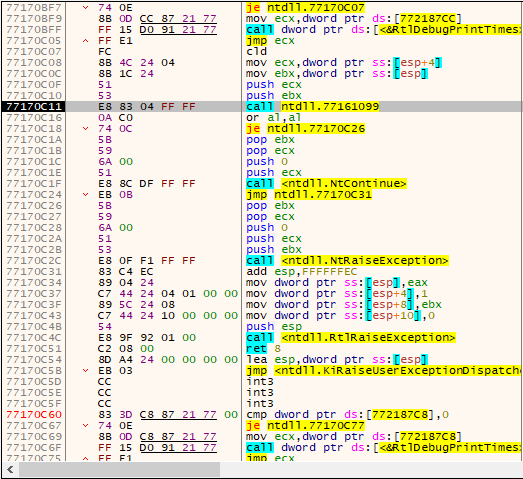
\includegraphics[width=3.5in]{network_function_call.png}
	\caption{call Instruction that Sends HTTP Messages}
	\label{fig:call_http}
\end{figure}


After looping through the code multiple times and trying to decipher the pattern in which the malware sends packets, I was finally able to find the function call that communicates with the server. Periodically it will perform a DNS query for the server and send the HTTP post message for the /api/register file. The exact call for the function is the following:

\begin{figure}[H]
\begin{Verbatim}
77170C11 | call ntdll.77161099
\end{Verbatim}
\caption{call Instruction to Send Messages to Command and Control Server}
\label{fig:net_function_call}
\end{figure}

\noindent The instruction sent the following messages to the Remnux virtual machine:

\begin{figure}[H]\centering
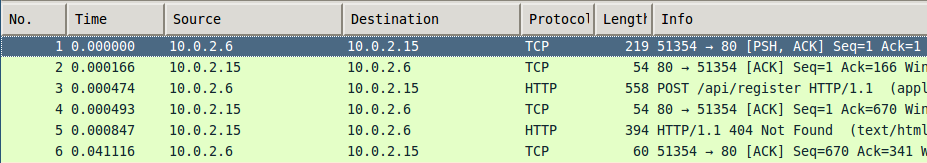
\includegraphics[width=\linewidth]{remnux_instruction_capture.png}
\caption{Remnux Wireshark Capture of Instruction}
\label{fig:remnux_instruction_cap}
\end{figure}

\newpage 


\subsection*{VII. Conclusions and Thoughts}


Given the amount of obfuscation within the code, Proteus is a hard malware to decipher. Without the command and control server there are a lot of untapped functions that are not being used, so it is difficult to fully access damages that can be caused by this piece of malware. Based on forumns and malware analysts, the malware is able to mine for cryptocurrency, log keystrokes, send commands and steal accounts. Though these functions remain untapped, we were still able to understand the basic functionality on how it is able to operate. Proteus runs three different processes all named chrome.exe. These processes either communicates with the command and control server or waits for a task to perform. Given the ability to access the network and manipulate processes on the infected host, it is easy to see how much these basic feautures can wreak havoc on a user. Not to mention the great use of ntdll.dll. Using this low-level kernel library the malware programmer made Proteus very difficult to reverse engineer. Given all this information, I hope to further investigate ntdll.dll and see if there is a possibility to determine what functions are being called using either ordinal numbers or addresses. 


\end{document}